\chapter{Introduction}\label{ch:Introduction}

Game Theory is the study of interactive decision making and developing
strategies through mathematics~\cite{Dictionary2013}. It analyses and gives
methods for predicting the choices made by players (those making a decision),
whilst also suggesting ways to improve their `outcome'~\cite{maschler_solan_zamir_2013}. Here, the abstract notion of utility is what
the players wish to maximise (see Chapter 2 in~\cite{maschler_solan_zamir_2013}
for a detailed discussion on the topic of utility theory or Section 1.3~\cite{Webb2007} for a more introductory explanation). One of the earliest
pioneers of game theory is mathematician, John von Neumann who, along with
economist Oskar Morgenstern, published \textit{The Theory of Games and Economic
Behaviour} in 1944~\cite{maschler_solan_zamir_2013}. This book discusses the
theory, developed in 1928 and 1940-41, by von Neumann, regarding ``games of
strategy" and its applications within the subject of economics~\cite{von2007theory}. Following this, several advancements have been made in the
area, including, most notably, John Nash's papers on the consequently named Nash
Equilibria in 1950/51~\cite{nash1950equilibrium, nash1951non}. Due to the
``context-free mathematical toolbox"~\cite{maschler_solan_zamir_2013} nature of
this subject, it has been applied to many areas, from
networks~\cite{liang2012game, 1593279} to biology~\cite{chen2009robust, adeoye2012application}. In this project, the main focus is on a
particular class of theorems, within game theory, known as ``Folk Theorems" with
application to the game of A Prisoner's Dilemma. These will be defined and
discussed in the subsequent sections.

\section{An Introduction to Games}\label{sec:An_Intro_to_Games}
Consider the following scenario:

\begin{center}
    Two convicts have been accused of an illegal act. Each of these prisoners,
    separately, have to decide whether to reveal information (defect) or stay
    silent (cooperate). If they both cooperate then the convicts are given a
    short sentence whereas if they both defect then a medium sentence awaits.
    However, in the situation of one cooperation and one defection, the prisoner
    who cooperated has the consequence of a long term sentence, whilst the other
    is given a deal.~\cite{Knight2017}
\end{center}

This is one of the standard games in game theory known as A Prisoner's Dilemma.
It has four distinct outcomes, for the given two player version, which can be represented as a table (see
Table~\ref{tab:PD_outcomes}).
\begin{tabular}{|c|}\label{tab:PD_outcomes}
    \hline
      &  & column player & \\
    \hline 
      &  & cooperate & defect\\
    \hline
    row player & cooperate & (3, 3) & (0, 5)\\
    \hline 
      &  & defect & (5, 0) & (1, 1)\\
    \hline
\end{tabular}
Each coordinate \((a, b)\) in the table represents the utility values obtained
for each player, where  \(a\) is the utility value obtained by the row player
and \(b\) is the utility gained by the column player. These utility values are
as given in \cite{axelrod1980effective} and are used throughout this project.
More formally, the game can be represented as the following matrix:

\kbordermatrix{
    \mbox{ } & coop & defect\\ 
    coop & (3, 3) & (0,5)\\ 
    defect & (5, 0) & (1, 1)
}\label{PDMatrix}

which is known as a \emph{normal form} representation of the game. The following
definition is adapted from~\cite{maschler_solan_zamir_2013}.

In general a \textit{normal form} or \textit{strategic form} game is defined by
an ordered triple \(G = (N, (S_i)_{i \in N}, (u_i)_{i \in N})\), where:
\begin{itemize}
    \item \(N = \{1, 2,..., n\}\) is a finite set of players;
    \item \(S = S_1 \times S_2, \times ... \times S_n\) is the set of strategies
    for all players in which each vector \((S_i)_{i \in N}\) is the set of
    strategies for player i \footnote{Since the game of A Prisoner's Dilemma has
    a finite strategy set for each player \(S_i = \{ \text{cooperate},
    \text{defect}\} (i \in N)\), in this project only finite strategy spaces are
    considered.}; and
    \item \(u_i : S \to \mathbb{R}\) is a payoff function which associates each
    strategy vector, \(\textbf{s} = (s_i)_{i \in N}\), with a utility
    \footnote{'Utility' is referred to as a player's `payoff' throughout the
    remainder of this report.} \(u_i(i \in N)\).
\end{itemize}

Yet another way of representing this game is as a pair of matrices, \(A, B\),
defined as follows:
\[
    A = 
    \begin{pmatrix}
       3 & 0\\
       5 & 1\\ 
    \end{pmatrix}
    \text{ and } B = A^{T}
    \begin{pmatrix}
        3 & 5\\
        0 & 1\\
    \end{pmatrix}
\]
This way of defining games allow for the use of calculating payoffs for each
player (see Section~\ref{sec:NE_for_Normal_Form_Games}).

Before continuing the discussion into the key notions of game theory, it needs
to be highlighted that there is an important assumption, which is central to
most studies of game theory, entitled \textit{Common Knowledge of Rationality}.
This, more formally, is an infinite list of statements which claim:
    \begin{itemize}
        \item The players are rational;
        \item All players know that the other players are rational;
        \item All players know that the other players know that they are rational; etc.    
    \end{itemize}
Assuming Common Knowledge of Rationality allows for the prediction of rational
behaviour through a processes entitled \textit{rationalisation}~\cite{Knight2019}
(see section 4.5 in~\cite{maschler_solan_zamir_2013} for an alternative
explanation of this assumption). 


A strategy for player \(i\), \(s_{i}\), is \textit{strictly dominated} if there
exists another strategy for player \(i\), say \(\bar{s_{i}}\), such that for all
strategy vectors \(s_{-i} \in S_{-i}\) of the other players, 
\[
    u_{i}(s_{i}, s_{-i}) < u_{i}(\bar{s_{i}}, s_{i}).
\]
In this case we say that \(s_{i}\) is \textit{strictly dominated} by
\(\bar{s_{i}}\). Here, \(s_{-i} = \{s_{1}, s_{2}, ..., s_{i-1}, s_{i+1}, ...,
s_{n}\}\), i.e. the \(i\)th player's strategy has been omitted. The set, \(S_{-i}\),
is defined similarly. Looking at the row player's matrix of a Prisoner's Dilemma
\ref{PDMatrix} (the first entries in the ordered tuples), it is clear that
cooperation is a strictly dominated strategy. Due to the symmetricity of the
game, this is also true for the column player.~\cite{maschler_solan_zamir_2013}



So far, only the pure strategies, \(S_{i}=\{\text{coop}, \text{defect}\}\), have
been discussed, thus the notion of a probability distribution over \(S_{i}\) is
now introduced, giving the so-called \textit{mixed strategies} as defined in~\cite{maschler_solan_zamir_2013}:
Let \(G=(N, (S_{i})_{i \in N}, (u_{i})_{i \in N})\) be a game (with each \(S_{i}\)
finite), then a \textit{mixed strategy} for player \(i\) is a probability
distribution over their strategy set \(S_{i}\). Define:
\[
\Sigma_{i} := \{\sigma_{i} : S_{i} \to [0, 1] : \sum_{s_{i} \in S_{i}}{\sigma_{i}(s_{i})} = 1\}   
\]
to be the set of mixed strategies for player \(i\). Hence, observe that the pure
strategies are specific cases of mixed strategies, with \(\sigma_{i} = (1, 0)\)
for cooperation and \(\sigma_{i} = (0, 1)\) for defection, in the example of a
Prisoner's Dilemma.

This leads onto the following definition of a \emph{mixed extension} of a game,
taken from~\cite{maschler_solan_zamir_2013}:
Let \(G\) be a finite normal form game as above, with \(S = S_{1} \times
S_{2} \times \cdots \times S_{N}\) defining the pure strategy vector set and
each pure strategy set, \(S_{i}\) being non-empty and finite. Then the
\textit{mixed extension} of \(G\) is denoted by
\[
    \Gamma = (N, (\Sigma_{i})_{i \in N}, (U_{i})_{i \in N}),
\]
and is the game in which, \(\Sigma_{i}\) is the \(i\)th player's strategy set
and \(U_{i} : \Sigma \to \mathbb{R}\) is the corresponding payoff function,
where each \(\sigma = (\sigma_{1}, \sigma_{2}, \ldots, \sigma_{N}) \in \Sigma =
\Sigma_{1} \times \Sigma_{2} \times \cdots \times \Sigma_{N}\) is mapped to the
payoff
\[
    U_{i} = \mathbb{E}_{\sigma}(u_{i}(\sigma)) = \sum_{(s_{1}, s_{2}, \ldots, s_{N}) \in S}{u_{i}(s_{1}, s_{2}, \ldots, s_{N})\sigma_{1}(s_{1})\sigma_{2}(s_{2})\cdots\sigma_{N}(s_{n})}
\]
for all players \(i \in N\).

\section{Nash Equilibrium for Normal Form Games}\label{sec:NE_for_Normal_Form_Games}
As mentioned above, mathematician, John Nash, introduced the concept of an
equilibrium point and proved the existence of mixed strategy Nash Equilibria in
all finite games. These notions are central to the study of game
theory~\cite{maschler_solan_zamir_2013} and hence, in this section, Nash's
concepts will be defined and proved in detail.

Firstly, before the definition of a Nash equilibrium, the idea, as given in~\cite{maschler_solan_zamir_2013} of a \textit{best response} is introduced:
For a game \(G=(N, (S_{i})_{i \in N}, (u_{i})_{i \in N})\), the strategy,
\(s_{i}\), of the \(i\)th player is considered a \textit{best response} to the
strategy vector \(s_{-i}\) if \(u_{i}(s_{i}, s_{-i}) = \max_{t_{i} \in
S_{i}}u_{i}(t_{i}, s_{-i})\).

This leads onto the main definition of the section:
\begin{definition}\label{def:NE}
    Given a game \(G=(N, (S_{i})_{i \in N}, (u_{i})_{i \in N})\), the vector of
    strategies \(s^{*} = (s_{1}^{*}, s_{2}^{*}, \ldots, s_{n}^{*})\) is a
    \textit{Nash equilibrium} if, for all players \(i \in N\), \(s_{i}^{*}\) is a best response to \(s_{i}^{*} \in N\).~\cite{maschler_solan_zamir_2013}
\end{definition}
In other words, \(s^{*}\) is a Nash equilibrium if and only if no player has any
reason to deviate from their current strategy \(s_{i}^{*}\).

Recall that, in Section~\ref{sec:An_Intro_to_Games}, for any player in A
Prisoner's Dilemma, defection dominated cooperation. This leads to the following
observation:
\begin{center}
    \textbf{The strategy pair (Defect, Defect), is the unique Nash equilibrium for A Prisoner's Dilemma, with a payoff value of 1 for each player.}~s\cite{maschler_solan_zamir_2013}
\end{center}
This can be visualised as followed:
Assume the row player uses the following mixed strategy, \(\sigma_{r} = (x,
1-x)\), i.e. the probability of cooperating is \(x\) and the probability of
defecting is \(1-x\). Similarly, assume the column player has 
the strategy, \(\sigma_{c} = (y, 1-y)\). The payoff obtained for the row and column player, respectively, is then:
\[
    A\sigma_{c}^T = \begin{pmatrix}
        3 & 0 \\
        5 & 1
    \end{pmatrix} \begin{pmatrix}
        y \\
        1-y
    \end{pmatrix} = \begin{pmatrix}
        3y \\
        4y + 1
    \end{pmatrix},

    \sigma_{r}B = \begin{pmatrix}
        3 & 5 \\
        0 & 1        
    \end{pmatrix} \begin{pmatrix}
        x & 1-x
    \end{pmatrix} = \begin{pmatrix}
        3x & 4x + 1
    \end{pmatrix}
\]

Plotting these gives the following:
\begin{figure}[h]
    \centering
        \begin{subfigure}[t]{0.45\textwidth}
        \centering
            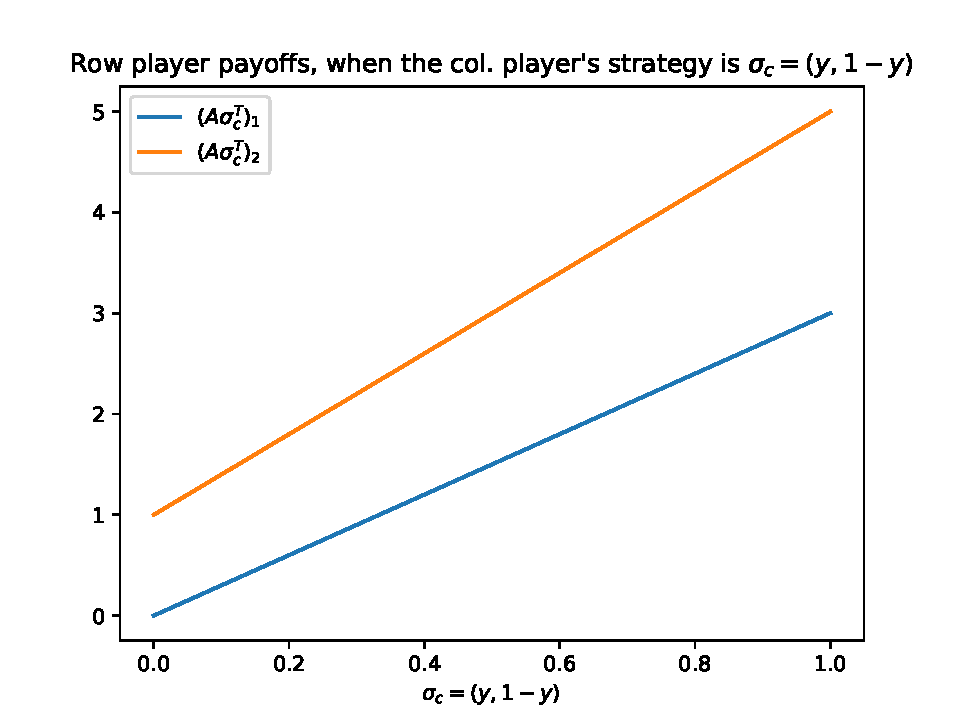
\includegraphics[width=\linewidth]{pd-row-payoff.pdf}
        \end{subfigure}
    \hfill
        \begin{subfigure}[t]{0.45\textwidth}
        \centering
            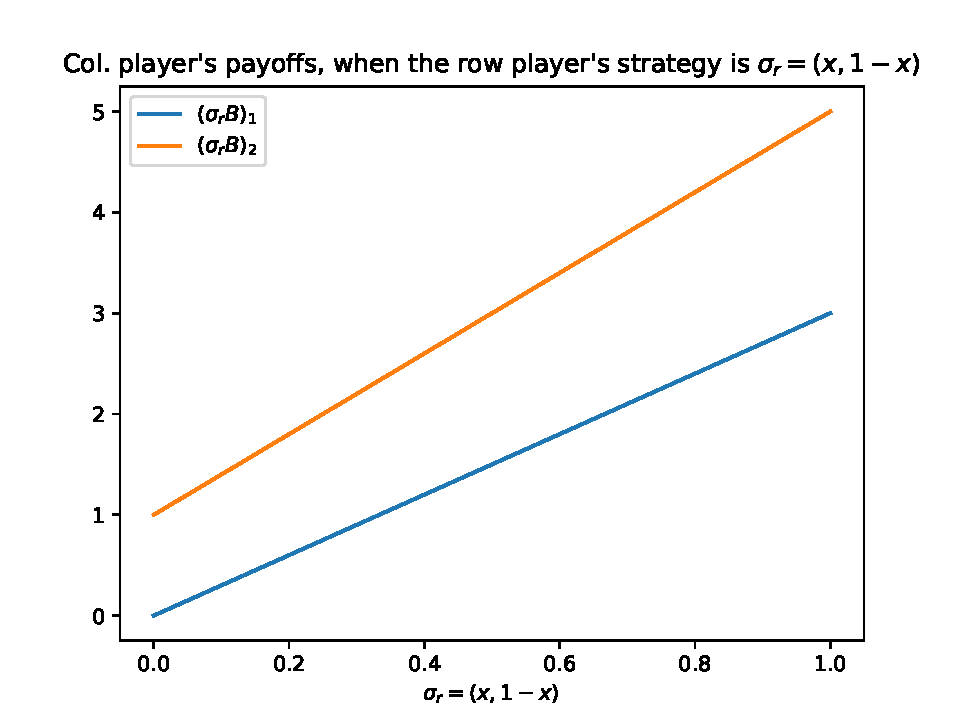
\includegraphics[width=\linewidth]{pd-col-payoff.pdf}
        \end{subfigure}~\caption{Graphs to show the row and column players' payoffs against a mixed strategy.}
    \label{fig:mixed_strategy_PD}
    \end{figure}
From Figure~\ref{fig:mixed_strategy_PD} it is clear that, regardless of the
strategy played by the opponent, defection is indeed the only rational move for
one to play. Thus, both players have no incentive to deviate if and only if both
play the strategy \(\sigma=(0, 1)\), i.e. defection for every single game of A
Prisoner's Dilemma.

On the other hand, consider, for example, a game with no dominated
strategies~\footnote{The game highlighted here is another standard used in game
theory entitled \emph{Matching Pennies}. Moreover, it is what is defined as a
\emph{zero-sum} game. Interested readers are encouraged to read Example 4.21
of~\cite{Webb2007} for an introduction to the game and Section 4.12
in~\cite{maschler_solan_zamir_2013} for an explanation of zero-sum games.}:
\[
    A =
    \begin{pmatrix}
        1 & -1\\
        -1 & 1\\
    \end{pmatrix}

    B =
    \begin{pmatrix}
        -1 & 1\\
        1 & -1\\
    \end{pmatrix}
\]
Are Nash Equilibria guaranteed to exist? This result is given in the next
theorem, taken from~\cite{nash1951non}, Nash's second paper on equilibria in games.

\begin{theorem}\label{thm:Nash}
    Every finite game has an equilibrium point.
\end{theorem}

The proof of Theorem~\label{thm:Nash} includes the use of a\emph{fixed point
theorem} and thus, a short sub-section regarding one such result is given, for
completeness, before providing a formal proof of~\ref{thm:Nash}.

\subsection{Brouwer's Fixed Point Theorem}\label{subsec:Brouwer_thm}
Brouwer's Fixed Point Theorem is a result from the theory of topology. Named
after the Dutch mathematician, L.E.J. Brouwer, it was proven in
1912~\cite{Carlson2016}. However, before stating this notion, a few conditions
regarding the properties of sets are recalled. 

The following three definitions appear as in~\cite{Weisstein, Barile, Weissteina} respectively:
\begin{definition}
    A set \(X \subseteq \mathbb{R}^{d}\) is called \textit{convex} if it
    contains all line segments connecting any two points \(\textbf{x}_{1},
    \textbf{x}_{2} \in X\).
\end{definition}

\begin{definition}
    An \textit{open cover} of a set \(S \subset X\), a topological space, is a
    collection of open sets \(A_{1}, A_{2}, \ldots \subset X\) such that
    \(A_{1} \cup A_{2} \cup \ldots \supset S\), that is, the union of the open
    sets contain S.
\end{definition}

\begin{definition}
    A subset \(S \subseteq X\), a topological space, is called \textit{compact}
    if, for each open cover of \(S\), there is a finite sub-cover of S.
\end{definition}

The presentation of Brouwer's Fixed Point Theorem is now given as in~\cite{maschler_solan_zamir_2013}
\begin{theorem}\label{thm:Brouwer}
    Let \(X \subseteq \mathbb{R}^{n}\) be a non-empty convex and compact
    set, then each continuous function \(f : X \to X\) has a fixed point.  
\end{theorem}
In other words if \(X\) and \(f\) satisfy the conditions given above then there
exists a point \(x \in X\) such that \(f(x) = x\). 

Since this project is regarding game theory, rather than topology, the proof to
the above theorem is omitted. However, the interested reader is referred
to~\cite{} for an in-depth consideration into the theory of topology.

\subsection{Proof of Nash's Theorem (Theorem~\ref{thm:Nash})}\label{subsec:Nash_Proof}
The proof provided here is adapted from the original, as presented
in~\cite{nash1951non}.

\begin{proof}
    NEED TO DO!!!!!!
\end{proof}

\section{Repeated Games}\label{sec:Repeated_Games}
The folk theorems studied in this project are a consequence of games which are
repeated several times (not just once). Thus, before discussing the main ideas,
the theory of both finitely- and infinitely- repeated games is presented.

However, firstly, a couple of alterations to the terminology used in
previous sections is redefined for conciseness and to be consistent with the literature~\cite{}.

What was known as a `game' will become known as a \emph{stage game} to highlight
the fact that a one-off game is being considered. Also, what was defined
previously as a `strategy' will now be referred to as an \emph{action} to
differentiate it from a strategy of a repeated game (see
Section~\ref{subsec:Finite_Repeated_Games}).

\subsection{Finite Repeated Games}\label{subsec:Finite_Repeated_Games}
According to~\cite{Knight2017a}, a \textit{\(T\)-stage repeated game}, \(T <
\infty\) is when the stage game, \(G\), is played \(T\) times, over discrete
time intervals. Each \(i\)th player has a strategy based on previous `rounds' of
the game and the payoff of a repeated game is calculated as the total sum of the
stage game payoffs.

Prior to giving the notion of a strategy in a repeated game, the idea of 
\emph{history}, within the context of repeated games, is provided.
The \textit{history}, \(H(t)\) of a repeated game is the knowledge of previous
actions of all players up until the \(t\)th stage game, assumed to be known by
player \(i\) for all \(i \in 1, \ldots, N\). Note that, when \(t=0\), \(H(0) =
\underbrace{(\emptyset, \emptyset, \ldots, \emptyset)}_{N \text{times}}\), since
no stage games have yet been played.

As given in~\cite{}, a \textit{strategy} of a \(T\)-stage repeated game is
defined to be a mapping from the complete history so far to an action of the
stage game, that is 
\[
    \tau_{i} : \cup_{t = 0}^{T-1}{H{t}} \to a_{i}. 
\]
Here, \(H(t)\) is the history of play as defined above and a_{i} is the \(i\)th
player's action of the stage game. 

Consider, for example, the repeated game in which the stage game of a Prisoner's
Dilemma is played each time. This is known as the \emph{Iterated Prisoner's
Dilemma} (IPD) and has been a popular topic of research for many years see
Chapter~\ref{ch:Literature_Search}.